\chapter{Wyniki i testy}
\label{cha:wyniki}

%TODO w miarę możliwości proszę spróbować się porównać z innymi pracami - jakaś tabelka, komentarz do wyników, ew. screeny
%+ tak jak w komentarzach poniżej - efekt filtracji, działanie śledzenia itp.

% Screeny i coś o tym dlaczego estymacja głębi nie działa
Po implementacji algorytmu w~języku Python sprawdzono jego działanie na dwa sposoby:
\begin{enumerate}
    \item Na różnych zbiorach danych z rzeczywistych kamer zdarzeniowych:
    \begin{itemize}
        \item Dla zbioru \textit{shapes rotation}, pochodzącego z~projektu \cite{dvs_dataset}. Jest to zbiór danych zarejestrowany przez przesuwanie i~obracanie kamerą zdarzeniową DAVIS240 nad powierzchnią z~umieszczonymi na niej różnorakimi kształtami. Nie są to dane zbliżone do tych, na których algorytm ma docelowo działać, lecz obecność wielu osobnych obiektów pozwala na ocenę segmentacji i~śledzenia.
        \item Dla zbioru \textit{night run}, pochodzącego z~projektu \cite{night_run}. Jest on dobrym sposobem na przetestowanie zdolności do wykrywania obiektów w~ciemności. Został stworzony przez zarejestrowanie człowieka biegnącego nocną porą przed obiektywem kamery zdarzeniowej zamocowanej na stojącym samochodzie.
    \end{itemize}
    % O ograniczeniach takiego testowania
    Testy na uprzednio zarejestrowanych zbiorach danych pozwalają na sprawdzenie działania tylko części algorytmu -- ponieważ nie ma w~nich dostępu do informacji o~parametrach zewnętrznych kamery (tj. pozycji i~orientacji), nie można przeprowadzić estymacji głębi.
    \item W~środowisku symulacyjnym Gazebo, gdzie mogą zostać przetestowane wszystkie etapy algorytmu. Testy zostały przeprowadzane dla różnych scenariuszy testowych, obejmujących:
    \begin{itemize}
        \item Sceny statyczne -- przeszkody, jakie obecne są na ścieżce drona, nie poruszają się względem otoczenia.
        \item Sceny dynamiczne -- przeszkoda to obiekt będący w ruchu.
    \end{itemize}
    W celu sprawdzenia działania algorytmu również przy ograniczonym oświetleniu, dla części sceny powtórzono test w~warunkach symulujących księżycową noc -- zachowano słabe źródło światła -- księżyc.
\end{enumerate}

\vspace{11px}
Niestety, po uruchomieniu symulacji i~odczytaniu wartości wyjściowych zauważono, że obliczane odległości drona do przeszkód nie są prawidłowe i~nie zachowują wystarczającej dokładności, żeby można było w~jakikolwiek sposób ich dalej użyć. Może być to spowodowane kilkoma czynnikami:
\begin{itemize}
    \item Metoda ta wymaga bardzo dokładnych danych o~pozycji i~rotacji kamery; dodatkowo muszą być one pobrane w~chwili wykrycia przeszkody,
    \item Błędy w~dopasowywaniu punktów charakterystycznych -- zdarzało się, że pary punktów nie były przypisane właściwie, co dodatkowo wpływało na przekłamania w~danych o~dystansie,
    \item Błędy w~procesie śledzenia obiektów -- aby metoda działała prawidłowo, wymagane są dane o~przeszkodzie z~bieżącej i~poprzedniej iteracji,
    \item Zbyt małe przemieszczenie drona między dwiema kolejnymi klatkami mogło wpłynąć na znaczne zmniejszenie dokładności -- nie sposób wyznaczyć głębię za pomocą triangulacji, jeśli dron nie przemieścił się względem przeszkody w żadnym kierunku.
\end{itemize}


Mimo wielu prób, nie udało się uzyskać poprawnych wyników, zachowując przyjętą metodę.
Brak prawidłowych danych o~dystansie do wykrytych obiektów jest poważnym problemem, który w~ostatecznej wersji algorytmu musi być rozwiązany w~inny sposób. % Potencjalne rozwiązania zaproponowano w~rozdziale \ref{sec:wnioski}.
Błąd uniemożliwia otrzymanie pozycji przeszkody w~trójwymiarowej przestrzeni, a~także powoduje niepoprawne wartości obliczanych prędkości przeszkód.

% Mimo błędnego działania ostatniej fazy algorytmu, możliwe jest przetestowanie wcześniejszych etapów i ocena jakości samej detekcji obiektów.

Algorytm realizuje zadanie detekcji obecności obiektów w~polu widzenia kamery zdarzeniowej. Dostarcza danych o~ich kształcie oraz rozmiarach i~położeniu na dwuwymiarowej płaszczyźnie obrazu. Możliwe jest przetestowanie wcześniejszych etapów i~ocena jakości samego wykrywania obiektów, pomimo błędnego działania ostatniej fazy algorytmu -- estymacji głębi.

\vspace{11px}
W pierwszej kolejności osobno sprawdzono działanie każdej z faz algorytmu.

% \vspace{11px}
% \noindent \textbf{Ocena jakości filtrowania}
% \vspace{11px}

Dzięki wizualizacji wyników filtrowania i~porównania go z oryginalnymi zdarzeniami, można ocenić jego jakość oraz dobrać parametry. Wynik działania filtru na symulacji z dodanym szumem można zobaczyć na rysunku \ref{fig:filter_example}.

% Porównanie frameów przed i po filtrowaniu - tylko jeden przykład
\begin{figure}
    \centering
    \begin{minipage}{0.5\textwidth}
        \centering
        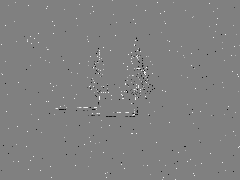
\includegraphics[width = 0.9\textwidth]{images/unfiltered_example.png}
    \end{minipage}\hfill
    \begin{minipage}{0.5\textwidth}
        \centering
        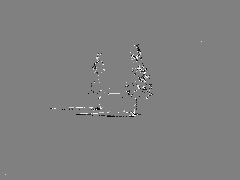
\includegraphics[width = 0.9\textwidth]{images/filtered_example.png}
    \end{minipage}
    \caption{Przykład ramki zdarzeniowej przed (po lewej) i po zastosowaniu filtracji (po prawej).}
    \label{fig:filter_example}
\end{figure}




% \vspace{11px}
% \noindent \textbf{Śledzenie przeszkód}
% może kilka kolejnych klatek z przeszkód - żeby pokazać, że są śledzone


% \vspace{11px}
% \noindent \textbf{Punkty charakterystyczne}
% Jeden screen z dopasowania cech


% \vspace{11px}
% \noindent \textbf{Testy na gotowych zbiorach danych}
% Zestawienia screenów dla zbioru danych z rzeczywistej kamery zdarzeniowej
\begin{figure}
    \centering
    \begin{minipage}{0.33\textwidth}
        \centering
        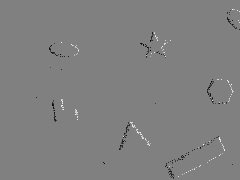
\includegraphics[width = 0.95\textwidth]{images/unfiltered_shapes1.png}
    \end{minipage}\hfill
    \begin{minipage}{0.33\textwidth}
        \centering
        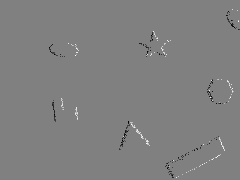
\includegraphics[width = 0.95\textwidth]{images/filtered_shapes1.png}
    \end{minipage}\hfill
    \begin{minipage}{0.33\textwidth}
        \centering
        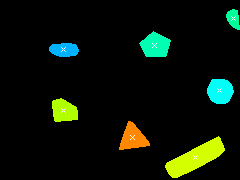
\includegraphics[width = 0.95\textwidth]{images/obst_shapes1.png}
    \end{minipage}
        \begin{minipage}{0.33\textwidth}
        \centering
        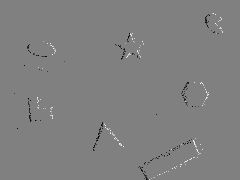
\includegraphics[width = 0.95\textwidth]{images/unfiltered_shapes2.png}
    \end{minipage}\hfill
        \begin{minipage}{0.33\textwidth}
        \centering
        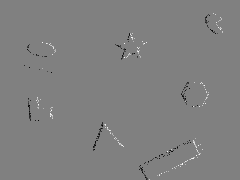
\includegraphics[width = 0.95\textwidth]{images/filtered_shapes2.png}
    \end{minipage}
    \begin{minipage}{0.33\textwidth}
        \centering
        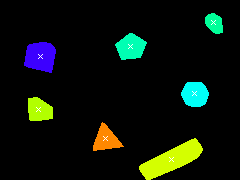
\includegraphics[width = 0.95\textwidth]{images/obst_shapes2.png}
    \end{minipage}\hfill
    \begin{minipage}{0.33\textwidth}
        \centering
        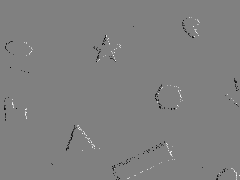
\includegraphics[width = 0.95\textwidth]{images/unfiltered_shapes3.png}
    \end{minipage}
        \begin{minipage}{0.33\textwidth}
        \centering
        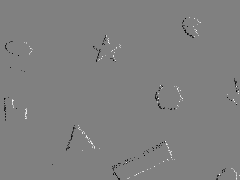
\includegraphics[width = 0.95\textwidth]{images/filtered_shapes3.png}
    \end{minipage}\hfill
    \begin{minipage}{0.33\textwidth}
        \centering
        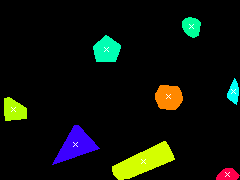
\includegraphics[width = 0.95\textwidth]{images/obst_shapes3.png}
    \end{minipage}\hfill
    \caption{Zestawienie wyników testowania algorytmu na zbiorze danych \textit{shapes rotation} w kilku wybranych momentach. Od lewej strony kolejne obrazki przedstawiają: dane przed filtracją, dane po filtracji, wykryte obiekty.}
    \label{fig:shapes_overview}
\end{figure}

\vspace{11px}

Jak można zauważyć na rysunku \ref{fig:shapes_overview}, zbiór danych \textit{shapes rotation} charakteryzuje się niewielkim szumem.
W śledzeniu obiektów czasem pojawiają się błędy -- szczególnie w przypadku zmiany kierunku ruchu obiektu. Jest to widoczne przez zmianę jego koloru. Obiekt również przestaje być śledzony, gdy znajdzie się poza polem widzenia, a następnie w nie powróci (SORT nie został wyposażony w funkcjonalność obsługującą takie przypadki). Nie jest to jednak duży problem -- algorytm wymaga jedynie możliwości porównania pozycji przeszkody z aktualnej i poprzedniej iteracji.

\vspace{11px}

Na podstawie rysunku \ref{fig:run_overview} można stwierdzić, że w~danych \textit{night run} występuje stosunkowo dużo szumu -- aby go wyeliminować, ustawiono bardziej rygorystyczne wartości parametrów filtra:
$$n=3; ~~t=\frac{1}{400}s; ~~k=6$$

W prostszym przypadku (tylko jeden poruszający się w jednym kierunku obiekt) nie występują żadne błędy w~śledzeniu -- przez cały test obiekt zachował ten sam kolor.


\begin{figure}
    \centering
    \begin{minipage}{0.33\textwidth}
        \centering
        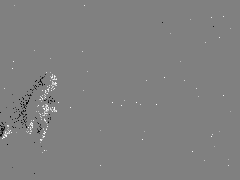
\includegraphics[width = 0.95\textwidth]{images/unfiltered_run1.png}
    \end{minipage}\hfill
    \begin{minipage}{0.33\textwidth}
        \centering
        
\includegraphics[width = 0.95\textwidth]{images/filtered_run1.png}
    \end{minipage}\hfill
    \begin{minipage}{0.33\textwidth}
        \centering
        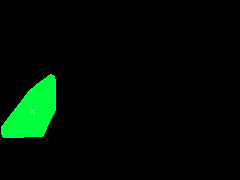
\includegraphics[width = 0.95\textwidth]{images/obst_run1.png}
    \end{minipage}
        \begin{minipage}{0.33\textwidth}
        \centering
        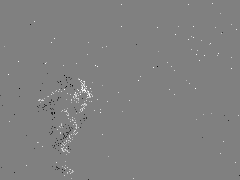
\includegraphics[width = 0.95\textwidth]{images/unfiltered_run2.png}
    \end{minipage}\hfill
    \begin{minipage}{0.33\textwidth}
        \centering
        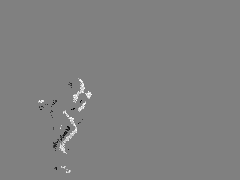
\includegraphics[width = 0.95\textwidth]{images/filtered_run2.png}
    \end{minipage}\hfill
    \begin{minipage}{0.33\textwidth}
        \centering
        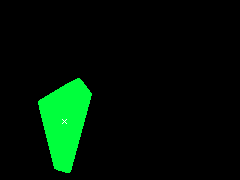
\includegraphics[width = 0.95\textwidth]{images/obst_run2.png}
    \end{minipage}
        \begin{minipage}{0.33\textwidth}
        \centering
        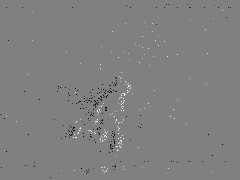
\includegraphics[width = 0.95\textwidth]{images/unfiltered_run3.png}
    \end{minipage}\hfill
    \begin{minipage}{0.33\textwidth}
        \centering
        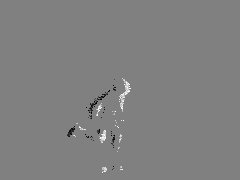
\includegraphics[width = 0.95\textwidth]{images/filtered_run3.png}
    \end{minipage}\hfill
    \begin{minipage}{0.33\textwidth}
        \centering
        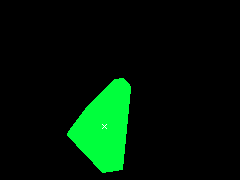
\includegraphics[width = 0.95\textwidth]{images/obst_run3.png}
    \end{minipage}
    \caption{Zestawienie wyników testowania algorytmu na zbiorze danych \textit{night run} w~kilku wybranych momentach. Od lewej strony kolejne obrazki przedstawiają: dane przed filtracją, dane po filtracji, wykryte obiekty.}
    \label{fig:run_overview}
\end{figure}


% \vspace{11px}
% \noindent \textbf{Scenariusze testowe w Gazebo}
% \vspace{11px}

\begin{figure}
    \centering
    \begin{minipage}{1\textwidth}
        \centering
        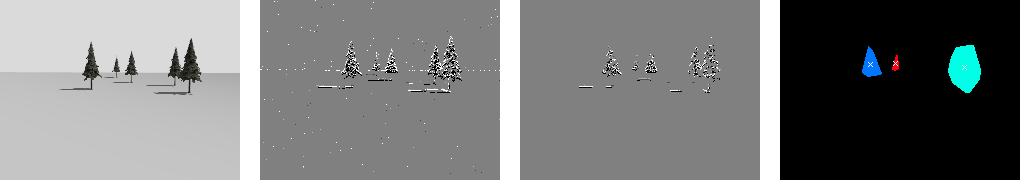
\includegraphics[width = 1\textwidth]{images/trees_day1.png}
    \end{minipage}
    \begin{minipage}{1\textwidth}
        \centering
        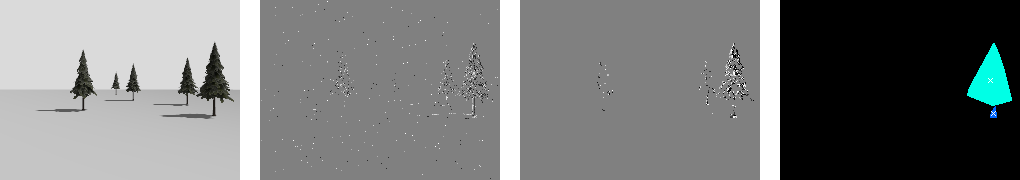
\includegraphics[width = 1\textwidth]{images/trees_day3.png}
    \end{minipage}
    \begin{minipage}{1\textwidth}
        \centering
        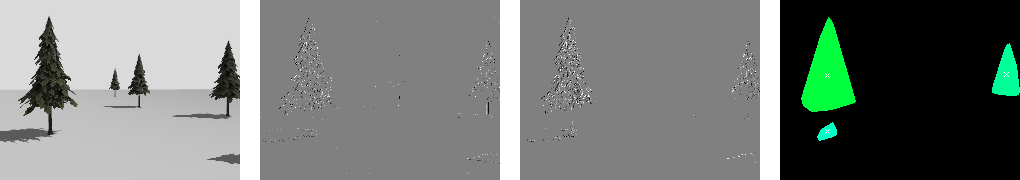
\includegraphics[width = 1\textwidth]{images/trees_day5.png}
    \end{minipage}
    \begin{minipage}{1\textwidth}
        \centering
        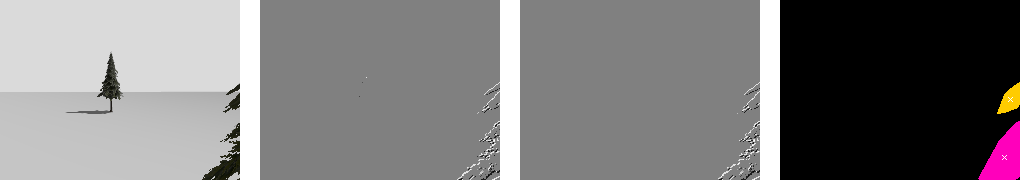
\includegraphics[width = 1\textwidth]{images/trees_day6.png}
    \end{minipage}
    \caption{Pierwszy scenariusz testowy -- statyczna scena w~dziennym świetle. Rolę przeszkód pełnią drzewa umieszczone przed lecącym naprzód dronem. Kolejne obrazki od lewej zawierają: obraz z~tradycyjnej kamery, nieprzefiltrowane dane z~DVS, dane z~DVS po filtracji, wykryte przeszkody.}
    \label{fig:trees_day}
\end{figure}

\vspace{11px}

 Na podstawie przebiegu testu sprawdzającego działanie systemu dla statycznej sceny w warunkach dziennych (rys. \ref{fig:trees_day}) można zauważyć kilka istotnych cech algorytmu:
 \begin{itemize}
     \item Algorytm często pomija przeszkody znajdujące się dalej i mające mniejszą prędkość względem drona -- jest to spowodowane głównie tym, że dane przetwarzane są w pakietach po $N$ zdarzeń. Jeśli w polu widzenia znajduje się przeszkoda, która generuje większość z nich, to zdarzenia związane z pozostałymi przeszkodami stanowią bardzo niewielką część całości, co powoduje, że są uznawane za szum -- jeśli nie na etapie filtracji, to podczas klasteryzacji. Nie jest to w jednoznaczny sposób wada -- pomijane w ten sposób przeszkody znajdują się daleko od drona i/lub poruszają się względem niego wolno. Algorytm nadaje priorytet tym, które stanowią większe zagrożenie.
     \item W przypadku gdy przeszkodami są drzewa, ich pień bywa uznawany za osobny obiekt. Podział jednej przeszkody na kilka osobnych obiektów prowadzi do niepotrzebnego wzrostu kosztu obliczeniowego.
     \item Obiekty, które w rzeczywistości znajdują się daleko od siebie, ale w klatce obrazu są blisko, uznawane są za jedną przeszkodę -- może to być jeden z czynników utrudniających triangulację.
 \end{itemize}

\begin{figure}
    \centering
    \begin{minipage}{1\textwidth}
        \centering
        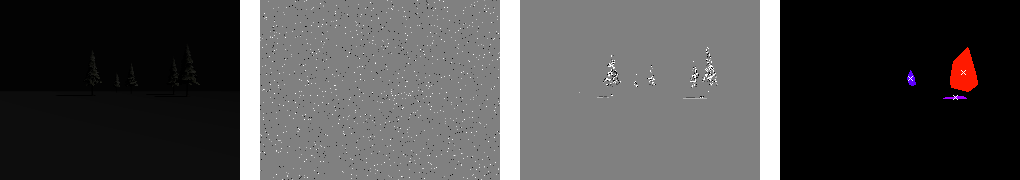
\includegraphics[width = 1\textwidth]{images/trees_night1.png}
    \end{minipage}
    \begin{minipage}{1\textwidth}
        \centering
        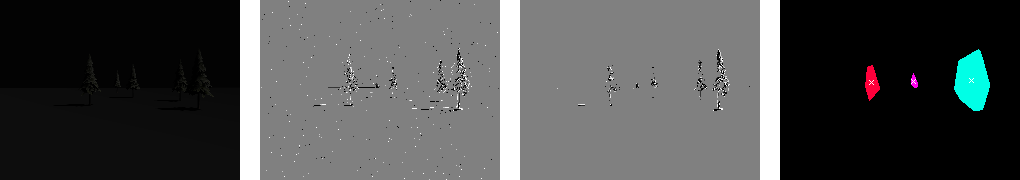
\includegraphics[width = 1\textwidth]{images/trees_night2.png}
    \end{minipage}
    \begin{minipage}{1\textwidth}
        \centering
        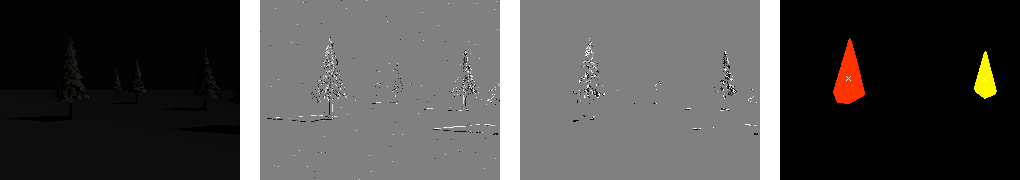
\includegraphics[width = 1\textwidth]{images/trees_night4.png}
    \end{minipage}
    \begin{minipage}{1\textwidth}
        \centering
        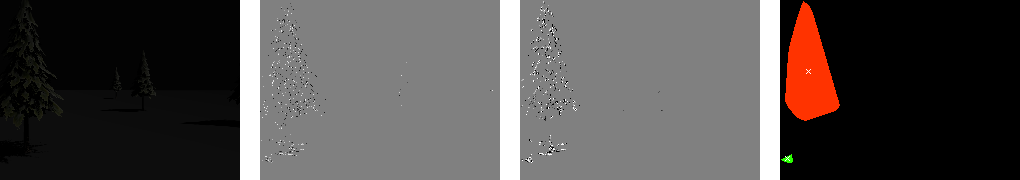
\includegraphics[width = 1\textwidth]{images/trees_night5.png}
    \end{minipage}
  
    \caption{Drugi scenariusz testowy -- statyczna scena w~nocy. Rolę przeszkód pełnią drzewa umieszczone przed lecącym naprzód dronem. Kolejne obrazki od lewej zawierają: obraz z~tradycyjnej kamery, nieprzefiltrowane dane z~ DVS, dane z~DVS po filtracji, wykryte przeszkody.}
    \label{fig:trees_night}
\end{figure}


Drugi scenariusz testowy (rys. \ref{fig:trees_night}) pokazuje, że nawet w ciemności algorytm zachowuje swoją funkcjonalność. Względem działania za dnia występują jednak pewne problemy:
\begin{itemize}
    \item Zdarza się, że jako przeszkoda rozpoznawana jest jedynie część rzeczywistego obiektu,
    \item Zaburzenia pracy algorytmu, takie jak utrata śledzonego obiektu i przypisanie do niego innego ID czy wykrycie cienia obiektu jako przeszkody, pojawiają się częściej.
\end{itemize}

\begin{figure}
    \centering
    \begin{minipage}{1\textwidth}
        \centering
        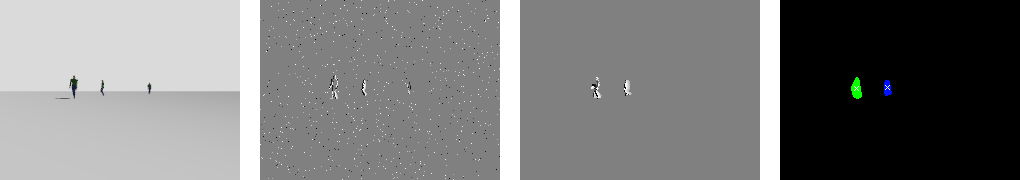
\includegraphics[width = 1\textwidth]{images/walk_day1.png}
    \end{minipage}
    \begin{minipage}{1\textwidth}
        \centering
        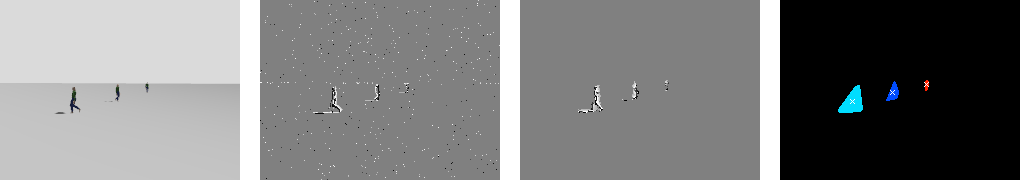
\includegraphics[width = 1\textwidth]{images/walk_day2.png}
    \end{minipage}
    \begin{minipage}{1\textwidth}
        \centering
        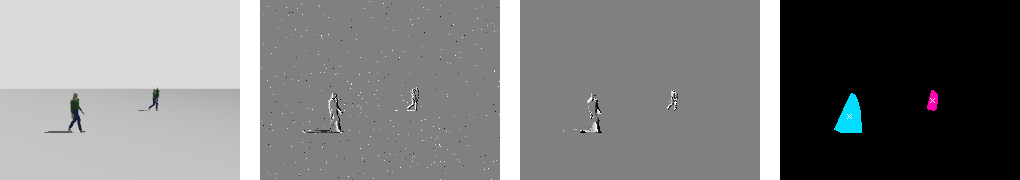
\includegraphics[width = 1\textwidth]{images/walk_day3.png}
    \end{minipage}
    \begin{minipage}{1\textwidth}
        \centering
        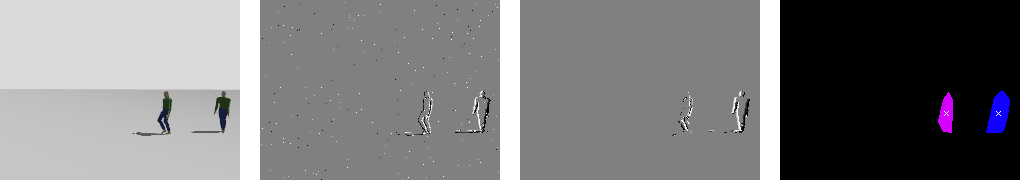
\includegraphics[width = 1\textwidth]{images/walk_day4.png}
    \end{minipage}
  
    \caption{Trzeci scenariusz testowy -- dynamiczna scena w dzień. Rolę przeszkód pełnią poruszające się szybkim krokiem ($1-1,5$ $m/s$) osoby. Kolejne obrazki od lewej zawierają: obraz z~tradycyjnej kamery, nieprzefiltrowane dane z~DVS, dane z~DVS po filtracji, wykryte przeszkody.}
    \label{fig:walk_day}
\end{figure}

\vspace{11px}

Na podstawie trzeciego testu (rys. \ref{fig:walk_day}) można stwierdzić, że poruszające się obiekty są wykrywane nawet skuteczniej niż te statyczne -- widoczne są z dalszej odległości.
Przyczyną tego jest większa liczba generowanych zdarzeń. Problemem, jaki można zaobserwować w~działaniu algorytmu, jest utrata ciągłości w śledzeniu przeszkód, gdy ludzie zmieniają kierunek ruchu lub wychodzą poza pole widzenia kamery.

\begin{figure}
    \centering
    \begin{minipage}{1\textwidth}
        \centering
        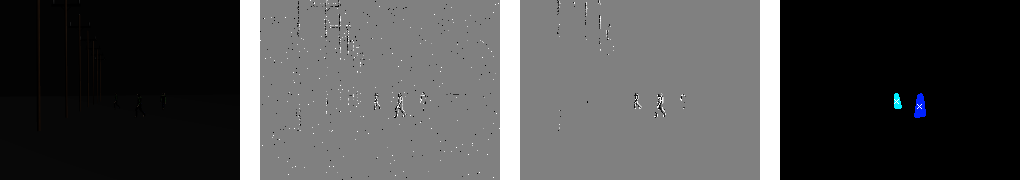
\includegraphics[width = 1\textwidth]{images/walk_night1.png}
    \end{minipage}
    \begin{minipage}{1\textwidth}
        \centering
        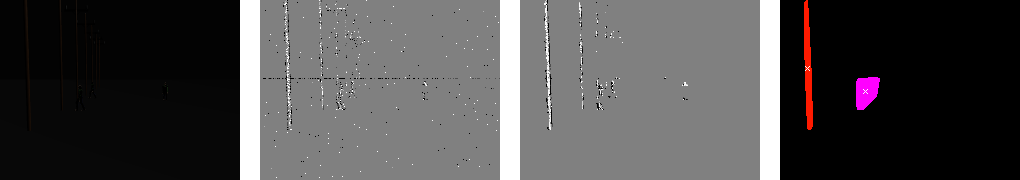
\includegraphics[width = 1\textwidth]{images/walk_night2.png}
    \end{minipage}
    \begin{minipage}{1\textwidth}
        \centering
        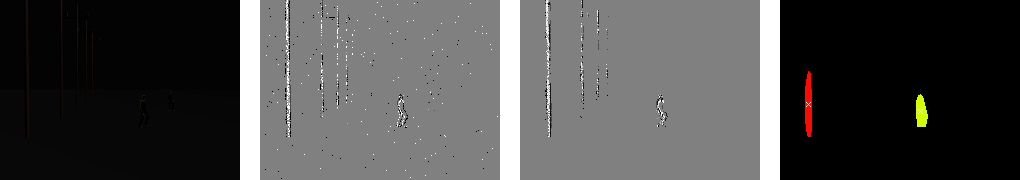
\includegraphics[width = 1\textwidth]{images/walk_night5.png}
    \end{minipage}
    \begin{minipage}{1\textwidth}
        \centering
        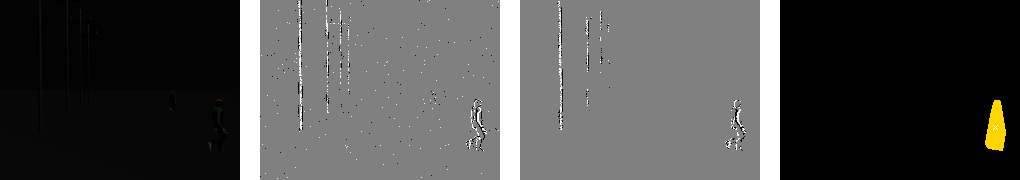
\includegraphics[width = 1\textwidth]{images/walk_night6.png}
    \end{minipage}
    \begin{minipage}{1\textwidth}
        \centering
        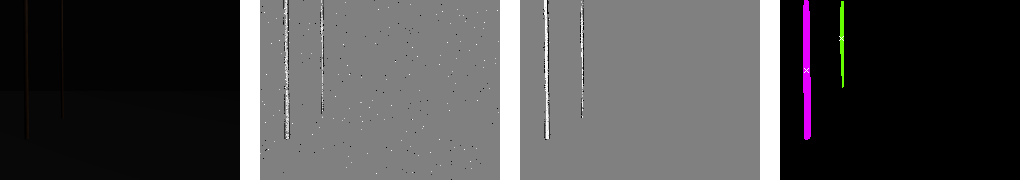
\includegraphics[width = 1\textwidth]{images/walk_night7.png}
    \end{minipage}
   
    \caption{Czwarty scenariusz testowy -- dynamiczna scena w nocy. Żeby utrudnić zadanie oprócz spacerujących ludzi, do sceny dodano rząd słupów energetycznych. Względem drugiego scenariusza (rys. \ref{fig:trees_night}), światła jest jeszcze mniej. Kolejne obrazki od lewej zawierają: obraz z tradycyjnej kamery, nieprzefiltrowane dane z DVS, dane z DVS po filtracji, wykryte przeszkody.}
    \label{fig:walk_night}
\end{figure}

\vspace{11px}
Z ostatnim, najtrudniejszym zadaniem (rys. \ref{fig:walk_night}), algorytm nie poradził sobie w pełni zadowalająco. W części klatek przeszkody nie były wykrywane lub były wykrywane tylko częściowo. Śledzenie obiektów stosunkowo często zawodziło -- co w znacznym stopniu utrudniałoby estymację głębi.

%Opis zalet i wad uzyskanego algorytmu
Na podstawie przeprowadzonych testów algorytmu można sformułować jego cechy -- zalety i~wady:
\begin{itemize}
    \item Gdy w~polu widzenia kamery znajduje się kilka obiektów, pośród których występują takie, które przez swoją większą prędkość lub bliższy dystans odpowiadają za generowanie wyższej liczby zdarzeń, pozostałe przeszkody nie są wykrywane. Zazwyczaj pomijane w~wyniku tego obiekty stanowią mniejsze zagrożenie dla drona, ponieważ poruszają się one wolno i/lub znajdują się daleko, więc takie zachowanie można potraktować jako zaletę -- ograniczana jest liczba wykrywanych obiektów, a~razem z~nią czas obliczeń.
    \item Algorytm dobrze radzi sobie w~ograniczonych warunkach oświetleniowych. Jak można zaobserwować na rysunkach \ref{fig:trees_night} oraz \ref{fig:walk_night}, w~pierwszej kolumnie obrazków widok z~tradycyjnej kamery jest całkowicie lub niemal całkowicie nieczytelny. Mimo to detekcja przeszkód ciągle jest możliwa, choć jej jakość nieco się zmniejsza.
    \item Typowe dla działania algorytmu błędy, których częstotliwość występowania nasila się w~bardzo trudnych warunkach oświetleniowych, to:
    \begin{itemize}
        \item Niewykrywanie obiektu na pojedynczych klatkach obrazu, co zaburza ciągłość jego działania i~powoduje dalsze błędy w śledzeniu przeszkód,
        \item Niewykrywanie całej przeszkody, a~tylko jej części -- problem dotyczy obiektów statycznych przy ograniczonym oświetleniu,
        \item Wykrywanie jednego obiektu jako kilka mniejszych przeszkód, co utrudnia śledzenie oraz może niepotrzebnie podwyższać czas potrzebny na przetwarzanie klatki.
    \end{itemize}
\end{itemize}
 


%---------------------------------%

